\chapter{Etat de l'art}
\paragraph*{} A rédiger
\section{Différents niveaux de chiffrements}
\paragraph*{} A rédiger
\section{Chiffrement de disque sur Linux et FreeBSD}
\paragraph*{} A rédiger
\subsection{Organisation dans le système d'exploitation}
\paragraph{}
Dans le cas de Linux, le chiffrement de disque est géré par le module noyau
{\em dm-crypt}, qui est un module qui dépend du module plus général
{\em device-mapper} qui gère les transformations de disque sous linux (RAID, 
LVM, Cache, ...). Le module dm-crypt gère la table appelée {\em crypt table}
qui permet d'associer un device à un chiffrement notamment. La table permet
la lecture des données sur le disque. A celà s'ajoute le programme cryptsetup
qui permet de lire des métadonnées stockées sur le disque pour remplir la {\em
crypt table}. Le programme s'occupe notamment du déchiffrement de la clé, de 
la lecture et de l'écriture des métadonnées sur le disque. L'organisation est 
donc la suivante :

\paragraph{}
\begin{figure}[h]
\centering
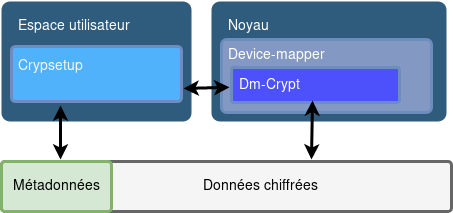
\includegraphics[width=.8\linewidth]{etat_art/organisation_linux.png}
\caption{\label{fig:OrgLinux}Organisation du code dans Linux}
\end{figure}

\paragraph{}
L'organisation reflétée par les programmes l'est également au niveau du code,
le module {\em dm-crypt} est agnostique de l'existance de métadonnées ainsi 
que de leur format. On a donc le module {\em device-mapper \em et \em dm-crypt}
qui font partie du code du noyau Linux, tandis que {\em Crypsetup} est un 
programme qui est fournit par linux en tant qu'utilitaire, qui est géré par 
une équipe indépendante de celle du noyau Linux. De plus {\em dm-crypt} est 
agnostique des algorithmes de chiffrement disponibles, le module s'appuie sur 
l'API de cryptographie du noyau.

\paragraph{}
Dans le cas de FreeBSD, le module noyau qui est en charge des
transformations sur les disques est {\em GEOM}. Comme sous linux, il existe des
modules qui vont interagir avec GEOM pour fournir des fonction de RAID, de 
cache, et également de chiffrement. Ces modules sont appelés {\em Classes GEOM}, 
celle qui fournit le chiffrement est nommée {\em ELI}, le module noyau associé 
est ainsi appelé {\em GELI}. Le module contrairement à {\em dm-crypt}, 
comprend toute la logique des métadonnées, ainsi que des algorithmes de 
chiffrement disponibles. L'outil en espace utilisateur tire son code directement
 du code du module {\em geli}. {\em GELI} profite de la connaissance du format 
des métadonnées pour directement détecter les partitions chiffrées, et donc 
proposer leur déchiffrement à l'utilisateur, là où Linux ne peut pas détecter de
partition ou disque chiffré, et c'est à l'utilisateur de préciser qu'il veut 
déchiffrer tel disque avec l'outil {\em crypsetup} qui va donc reconnaître le 
format.


\subsection{Format sur disque}
\paragraph{}
Le format sur disque désigne l'organisation des données et métadonnées sur le 
disque. L'idée générale étant de stocker sur une partie du disque les 
informations permettant de déchiffrer une autre partie du disque.
\paragraph{}
Comme le noyau Linux ne contient pas de format de métadonnées, 
c'est {\em Crypsetup} qui a choisi de créer un format appelé {\em Linux 
Unified Key Setup (LUKS)}, comme format standard pour le chiffrement de disque 
sous Linux. En effet, {\em Crypsetup} implémente d'autres format de 
métadonnées comme {\em TrueCrypt} développé par la {\em TrueCrypt Fondation}. 
Le format LUKS consiste en des métadonnées au début de la partition, précédant 
les données chiffrées.

\paragraph{}
\begin{figure}[h]
\centering
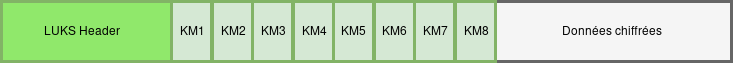
\includegraphics[width=.8\linewidth]{etat_art/format_disque_luks.png}
\caption{\label{fig:LUKSFormat}Format sur disque LUKS}
\end{figure}

\paragraph{}
Les métadonnées de LUKS contenant les algorithmes de chiffrement, 
d'authentification, la version de LUKS, sont suivis de huit emplacements 
permettant de stocker des clés chiffrées, qui permettent de déchiffrer le 
disque. Ainsi on peut stocker la même clé huit fois, protégées par des mots de 
passe différents, permettant ainsi à plusieurs utilisateurs de déchiffrer le 
même disque sans pour autant partager le même mot de passe.

\paragraph{}
Les métadonnées de GELI sont stockées contrairement à LUKS, à la fin du disque.
L'en-tête permet de stocker 2 clés, et s'étend sur un seul secteur.


\paragraph{}
\begin{figure}[h]
\centering
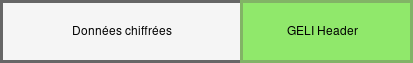
\includegraphics[width=.5\linewidth]{etat_art/format_disque_geli.png}
\caption{\label{fig:GELIFormat}Format sur disque GELI}
\end{figure}

\paragraph{}
Dans les deux en-têtes on retrouve des champs similaires, un {\em Magic} qui 
permet de connaître le type d'en-tête, la version, l'algorithme de chiffrement 
et d'authentification, etc. On peut noter tout de même que la taille de 
l'en-tête sous GELI fait 255 octets, contre 592 octets pour LUKS.



\subsection{Algorithmes}
\subsubsection{Algorithmes de chiffrement}
\paragraph{}
Les algorithmes de chiffrement disponibles pour GELI \cite{geli.h} sont :
\begin{itemize}
	\item Null
	\item Null-CBC
	\item AES-CBC
	\item AES-XTS
	\item Blowfish
	\item Blowfish-CBC
	\item Camellia
	\item Camellia-CBC
	\item 3DES
	\item 3DES-CBC
\end{itemize}

\paragraph{}
Dans le cas de {\em LUKS}, la spécification \cite{onDiskFormatLuks}
ne précise pas la liste des algorithmes disponibles, la liste des algorithmes 
possibles est laissée ouverte pour permettre l'utilisation de tout ceux que le 
noyau Linux peut mettre à disposition via son API.

\subsubsection{Utilisation de la clé primaire}
\paragraph{}
Dans le cas de LUKS, la spécification \cite{onDiskFormatLuks} précise que la 
clé stockée dans l'en-tête LUKS est utilisée directement comme clé de 
chiffrement. Dans le cas de GELI, la clé est dérivée selon un algorithme 
déterministe en des clé utilisée pour chiffrer les données, qui dépendent de 
la version de GELI et de l'utilisation d'authentification des données 
\cite{manGeli}. La version 5 de GELI utilisait une seule clée, qui était la clé
primaire fournit par les métadonnées, à partir de la version 6, la clé primaire
est dérivée en clé de chiffrement, qui diffèrent tout les 2\textasciicircum20 
secteurs, soit 1048576 secteurs du disques. Les tailles des secteurs des 
disques étant généralement de 512 octets ou 4096 octets, 
donc tout les 500Mo ou 4Go environ.
La taille du secteur correspond au champs taille du secteur des métadonnées
GELI.

\subsubsection{Algorithmes d'authentification (HMAC)}
\paragraph{}
Les algorithmes d'authentification disponibles sous GELI sont:
\begin{itemize}
	\item MD5
	\item SHA1
	\item Ripemd160
	\item SHA256
	\item SHA384
	\item SHA512
\end{itemize}

\paragraph{}
Tandis qu'encore une fois pour LUKS, la liste des algorithmes autorisée, n'est 
pas précisée, c'est donc celle que le noyau Linux peut mettre à disposition 
qui est disponible.

\subsection{Fonctionnalités}
\paragraph{}
Les deux systèmes de chiffrement : {\em dm-crypt \em et \em geli} profitent 
de l'accélération matérielle pour les opérations de chiffrement grâce au 
noyau (AES-NI notamment). LUKS supporte l'hibernation sur disque 
contrairement à GELI, qui ne le supporte pas car FreeBSD ne supporte pas 
l'hibernation sur disque. Les deux systèmes permettent le renforcement de 
phrases de passe, via la fonction {\em PBKDF2} décrite par le standard 
{\em PKCS\#5v2}. Les deux formats de métadonnées permettent l'utilisation de 
plusieurs clés.

\subsubsection{Intégration avec la séquence de démarrage}
\paragraph{}
L'intégration avec le démarrage permet notamment d'avoir la racine du système 
de fichier sur une partition chiffrée, et même éventuellement le {\em /boot}
dans lequel sont usuellement stockés les fichiers permettant de démarrer le 
système d'exploitation.

\paragraph{}
Dans le cas de Linux, le format LUKS a été intégré dans l'initramfs via un
hook qui charge le module dm-crypt puis utilise le binaire cryptsetup pour 
déchiffrer le disque. Le format LUKS a également été intégré à GRUB sous la 
forme du module {\em luks.mod}. Il permet au premier stage de GRUB de 
déchiffrer la partition sur laquelle se trouve la configuration de GRUB.
Ainsi sous Linux, il est possible de chiffrer toute la racine de son système,
{\em /boot} compris. Il est ensuite question de pouvoir taper un seule fois la 
phrase de passe, pouvoir faire de l'authentification unique (SSO), cela est 
également possible, il suffit de mettre un fichier contenant la clé de 
chiffrement en clair dans l'initramfs. Ainsi GRUB déchiffre le disque, 
puis charge l'initramfs qui peut déchiffrer la partition sans avoir besoin 
de demander une phrase de passe.

\paragraph{}
Dans le cas de GELI, il est également possible de chiffrer la racine du 
système, le bootloader de FreeBSD étant capable de lire les métadonnées GELI, 
ainsi que de déchiffrer des données. Il est également possible de chiffrer le 
{\em /boot} car le 2ème stage du bootloader ({\em boot2}) contient le code 
nécessaire pour déchiffrer un disque au format GELI, à condition que la table 
de partition soit au format GPT. La phrase de passe est passée via une zone 
mémoire au dernier stage qui pourra l'utiliser pour démarrer.

